\documentclass{report}

\usepackage[utf8]{inputenc} % Charakter-Kodierung
\usepackage[german]{babel} % Sprache

\usepackage[table,xcdraw]{xcolor} % Tabellen Farben
\usepackage{tabularx} % Dynamische Tabellenbreite
\usepackage{tcolorbox} % Graue Boxen
\usepackage{hyperref} % url Umgebung
\usepackage{todonotes} % Notizen
\usepackage{natbib} % Bibliographie
\usepackage{fancyhdr} % Header und Footer
\usepackage{multirow} % Multizeile
\usepackage{geometry} % Page layout
\usepackage{color} % Text Farben
\usepackage[section]{placeins}%Stops pictures from moving around EVERYWHERE

% Page layout
\geometry{
	bottom=3.5cm,
	headheight=180pt
}

% Nummerierung der ersten Seiten verhindern
\pagenumbering{gobble}

% Bibstyle
\bibliographystyle{plain}

% Header / Footer
\fancypagestyle{plain}{
	\fancyhf{}% Clear header/footer
	\fancyhead[R]{\includegraphics[width=4cm]{img/cau-logo-2017}} % Rechter header
	\fancyhead[L]{\leftmark} % Linker header
	\fancyfoot[R]{\thepage} % Rechter footer
	\fancyfoot[L]{
\includegraphics[width=1cm]{img/se-logo}} % Linker footer	
}
\pagestyle{plain}

\renewcommand{\headrulewidth}{0.5pt} % Unnötige Informationen der Kapitelangabe
\renewcommand{\footrulewidth}{0.2pt} % entfernen
\renewcommand{\chaptermark}[1]{\markboth{{#1}}{}}




% Zahlen für Fußnoten
\renewcommand{\thefootnote}{\arabic{footnote}}
\renewcommand{\thempfootnote}{\arabic{mpfootnote}}

%%%%% Ausfüllen %%%%%

% Gruppenname
\newcommand{\gruppenname}{WSP31}

% Projektname
\newcommand{\projektname}{SWARM Composer}

% Semester
\newcommand{\semester}{SoSe18}



% Titelseite

\title{
	\vspace*{-3cm}
	Entwurfsdokumentation\\
	\projektname\\
	-\\
	\color{gray}
	Softwareprojekt \semester\\
	\gruppenname\\
	\vspace*{5mm}
	
\includegraphics[width=\textwidth]{img/Logo}
}

\author{
	\begin{tabular}{r l@{\hspace{8\tabcolsep}} r} 
		Lorenz & Boguhn & \multirow{8}{*}{ 
\includegraphics{img/se-logo} } \\
		Lennart & Brandt \\
		Arved & Hansen \\
		Matthias & Johannsen \\
		Lars & Jürgensen \\
		Birger & Thormählen \\
		Björn & Vonheiden\\
		Thomas & Zacher \\
	\end{tabular}
}

\date{\today}





% Dokument

\begin{document}
	
	\maketitle

	\tableofcontents 
	
	\chapter{Einleitung}\label{chp:einleitung}
	\pagenumbering{arabic} % Nummerierung starten
	\thispagestyle{fancy}
	\section{Dokumentaufbau}\label{sec:dokumentaufbau}
In dieser Entwurfsdokumentation beschreiben wir die technische Ausführung, der im Pflichtenheft beschriebenen Funktionen, des SWARM Composers. Hierfür stellen wir erst die Komponenten dar und zeigen dann, wie diese später auf der Hardware verteilt werden.
Danach beschreiben wir mithilfe mehrerer Klassendiagramme die innere Struktur unserer Software.
Im fünften Kapitel, in den Sequenzdiagrammen, spezifizieren wir die detaillierte Ausführung komplexer Anwendungsfälle.
Weiter haben wir unsere API-Schnittstelle designet auf die die Clients zugreifen.
Zum Abschluss erklären wir im Glossar noch einige Abkürzungen und Begriffe.

\section{Zweckbestimmung}\label{sec:zweckbestimmung}
Das Produkt soll einem die Möglichkeit bieten sich schnell über die Kompatibilität von verschiedenen Produkten zu informieren.
Dabei soll das System besonders leicht und intuitiv bedienbar sein.
Um dies zu verwirklichen, ist die Webseite speziell darauf ausgelegt, passende Kombinationen zu entwickeln und Inkompatibilitäten leicht durch Alternativen zu ersetzten.
Im Gegensatz dazu ist die App für Präsentationen von Diensten und Kombinationen konzipiert.
Zudem ist es ein Ziel die Verwaltung der Produkte leicht zu gestalten.

\section{Entwicklungsumgebung}\label{sec:entwicklungsumgebung}

\begin{table}[h]
	\centering
	\begin{tabularx}{\textwidth}{l l X}
		\rowcolor[HTML]{C0C0C0}
		\textbf{Software} & \textbf{Version} & \textbf{URL} \\
		Docker & 17.03.2-ce & \url{https://www.docker.com} \\	
		\rowcolor[HTML]{E7E7E7}
		Git & - & \url{https://git-scm.com} \\
		GitLab & - & \url{https://git.informatik.uni-kiel.de} \\	
		\rowcolor[HTML]{E7E7E7}			
		Java Development Kit & 8u144 & \url{http://www.oracle.com/technetwork/java/javase/downloads/index.html} \\
		Jenkins & - & \url{http://134.245.1.240:9002} \\		
		\rowcolor[HTML]{E7E7E7}
		Jira & - & \url{http://maui.se.informatik.uni-kiel.de:58080} \\
		Tomcat & - &  \url{http://134.245.1.240:9001} \\
	\end{tabularx}
	\caption{Enwicklungsumgebung und Tools allgemein}
	\label{table:entwicklungsumgebung-allgemein}
\end{table}

\begin{table}[h]
	\centering
	\begin{tabularx}{\textwidth}{l l X}
		\rowcolor[HTML]{C0C0C0}
		\textbf{Software} & \textbf{Version} & \textbf{URL} \\
		Bootstrap & 4.1.1 &  \url{https://getbootstrap.com/} \\
		\rowcolor[HTML]{E7E7E7}
		Fabric.js & 2.3.6 &  \url{http://fabricjs.com/} \\
		IntelliJ IDEA Ultimate & 2018.2 & \url{https://www.jetbrains.com/idea/} \\		
		\rowcolor[HTML]{E7E7E7}
		jQuery & 3.3.1 &  \url{https://jquery.com} \\
		Maven & 3.5.4 & \url{https://maven.apache.org} \\
		\rowcolor[HTML]{E7E7E7}
		Spring Boot & 2.0.4 & \url{https://spring.io/projects/spring-boot} \\
		Spring Framework & 5.0.8 & \url{https://spring.io/projects/spring-framework} \\
		\rowcolor[HTML]{E7E7E7}
		Thymeleaf & 3.0.9 & \url{https://www.thymeleaf.org} \\
	\end{tabularx}
	\caption{Enwicklungsumgebung Webapplikation}
	\label{table:entwicklungsumgebung-server}
\end{table}

\begin{table}[h]
	\centering
	\begin{tabularx}{\textwidth}{l l X}
		\rowcolor[HTML]{C0C0C0}
		\textbf{Software} & \textbf{Version} & \textbf{URL} \\
		Android Studio & 3.1.4 & \url{https://developer.android.com/studio/} \\
		\rowcolor[HTML]{E7E7E7}
		Gradle & 4.10 & \url{https://gradle.org} \\
	\end{tabularx}
	\caption{Enwicklungsumgebung App}
	\label{table:entwicklungsumgebung-app}
\end{table}

	
	\chapter{Komponentendiagramme}\label{chp:komponentendiagramme}
	\thispagestyle{fancy}
	\section{Server}
\begin{figure}[h]
	\centering
	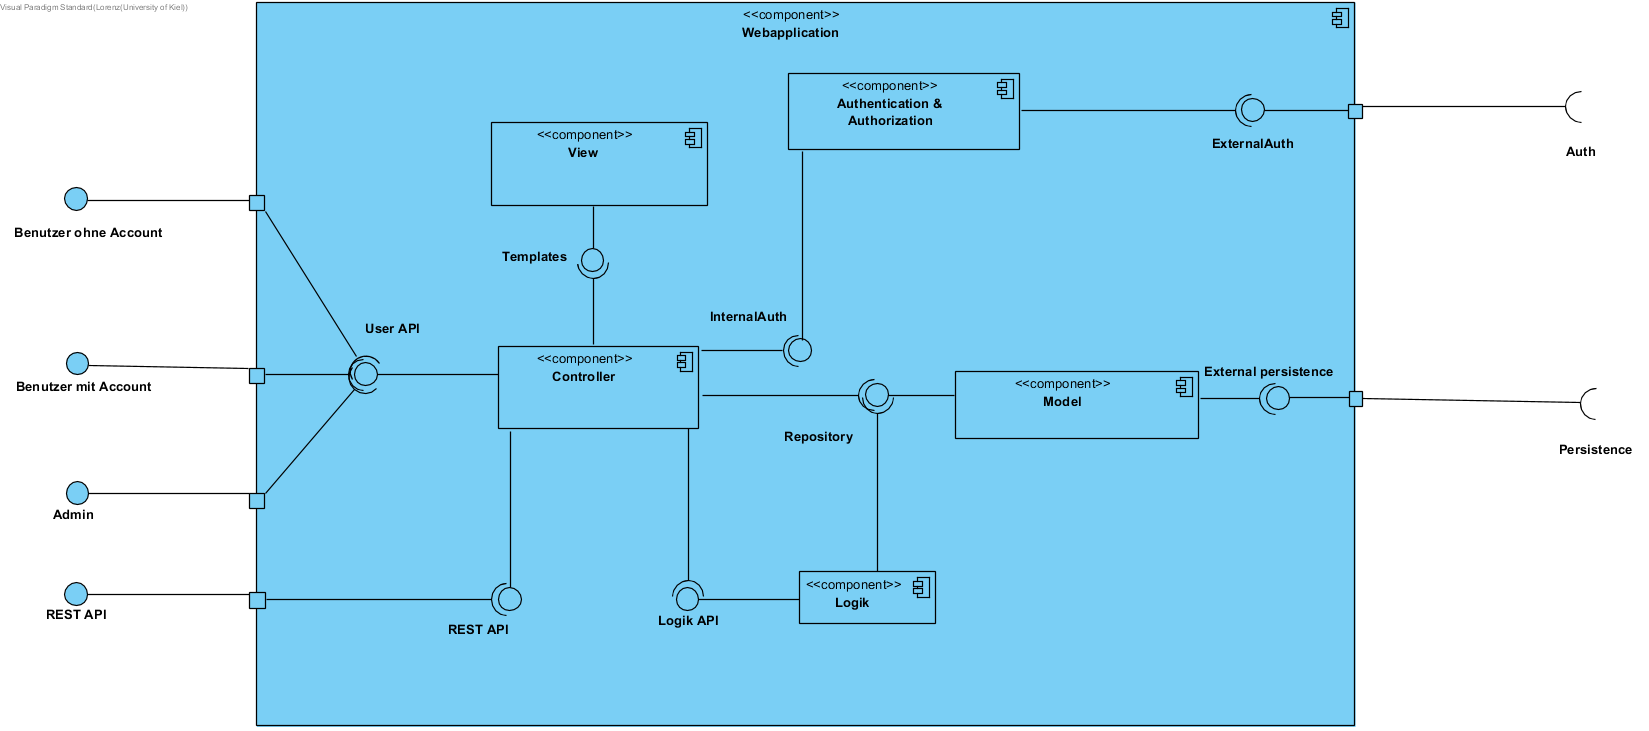
\includegraphics[width=\textwidth]{komponentendiagramm/Server}
	\caption{Komponentendiagramm - Server}
	\label{fig:komponentendiagramm-server}
\end{figure}

\begin{table}[h]
	\centering
	\begin{tabularx}{\textwidth}{X X}
		\rowcolor[HTML]{C0C0C0}
		\textbf{Komponentenname} & \textbf{Aufgabe} \\
		Authentification \& Authorization & Authentifizierung und Logins/Logouts\\
		\rowcolor[HTML]{E7E7E7}
		Controller & Beantwortet Anfragen von außen und übernimmt die interne Kommunikation\\
		Logik & Berechnet Lösungen für Anfragen, die über die einfache Logik des Controllers hinaus geht\\
		\rowcolor[HTML]{E7E7E7}
		Model & Enthält alle Daten aus der DB und bietet sie über eine Schnittstelle an\\
		View & View bereitet die Daten in einer HTML Seite auf und enthält Funktionalität für die Webseite
	\end{tabularx}
	\caption{Subkomponentenbeschreibung - Server}
	\label{table:Subkomponentenbeschreibung - server}
\end{table}

\FloatBarrier
Die meisten Schnittstellen aus dieser Abbildung werden bereits durch das Spring-Framework bereitgestellt.
In diesem System stellen die Webseitennutzer über die User API Anfragen an den Controller.
Die App-Nutzer nutzen dafür die REST API.
Der Controller wertet die Anfrage aus und bearbeitet diese mit Hilfe der anderen Komponenten.
Dabei ist die Authentification \& Authorization-Komponente dafür zuständig, zu überprüfen ob eine Anfrage authentifiziert ist und auch für Logins und Logouts.
Die View-Komponente ist hier bei für die Aufbereitung der Informationen in HTML zuständig. Weiter ist dort Funktionalität/Logik für die Browserwebseite mit enthalten.
In der Logik-Komponente werden komplexere Berechnungen durchgeführt.
So werden hier beispielsweise Alternativen für inkompatible Verbindungen.
Die Model-Komponente ist lediglich für die Datenverwaltung und die Kommunikation mit der DB zuständig.
Dafür stellt die Model-Komponente die Repository-Schnittstelle bereit.

\section{App}
\begin{figure}[h]
	\centering
	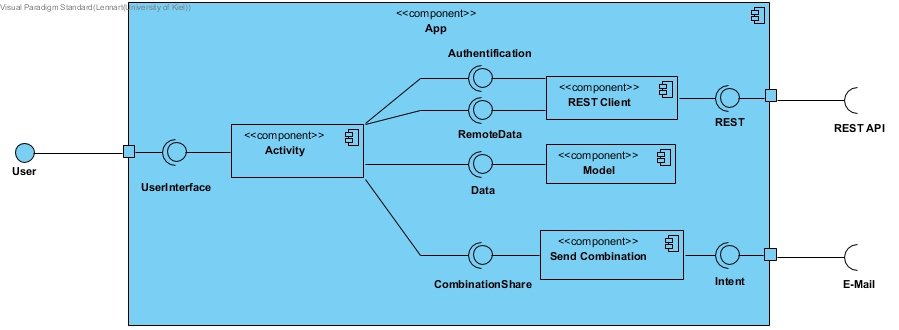
\includegraphics[width=\textwidth]{komponentendiagramm/App}
	\caption{Komponentendiagramm - App}
	\label{fig:komponentendiagramm-app}
\end{figure}

\begin{table}[h]
	\centering
	\begin{tabularx}{\textwidth}{X X}
		\rowcolor[HTML]{C0C0C0}
		\textbf{Komponentenname} & \textbf{Aufgabe} \\
		Activity & Darstellung der App Oberflächen und Schnittstelle für den Benutzer\\
    \rowcolor[HTML]{E7E7E7}
		 Model & Modelliert die Daten, die von der REST API zur Verfügung gestellt werden\\
		 REST Client & Kommunikation zwischen REST API und der App\\
    \rowcolor[HTML]{E7E7E7}
		Send Combination & Generiert PDF und leitet dies weiter an Standard E-Mail Programm
	\end{tabularx}
	\caption{Subkomponentenbeschreibung - App}
	\label{table:Subkomponentenbeschreibung - app}
\end{table}

Die App Komponente modelliert die zu entwickelnde App.
Der User interagiert dabei über das User Interface mit der Anwendung.
Die Activity Komponente nimmt dabei die Interaktionen entgegen und führt dementsprechend Aktionen aus.
Dabei besteht die Activity Komponente aus der Darstellung, die bei Android über XML stattfindet und den eigentlichen Activities, die die Interaktionen entgegennehmen.
Von den Activities aus werden die REST Client, Model und Send Combination Komponenten verwendet.
\\
Der REST Client bietet einerseits eine Schnittstelle für die Authentifikation und für das Einloggen und anderseits eine, um Daten von dem Server zu holen.
\\
Die Model Komponente modelliert die benötigten Daten in der App.
Die Klassen im Model entsprechen den Daten von der REST API.
\\
Die Send Combination Komponente ermöglicht das Teilen von Kombinationen.
Dabei wird die Kombinationen und ein beschreibender Text zu einem PDF umgewandelt und dann über eine Schnittstelle an einen E-Mail Client weitergegeben.

	
	\chapter{Verteilungsdiagramm}\label{chp:verteilungsdiagramm}
	\thispagestyle{fancy}
	\begin{figure}[ht]
	\centering
	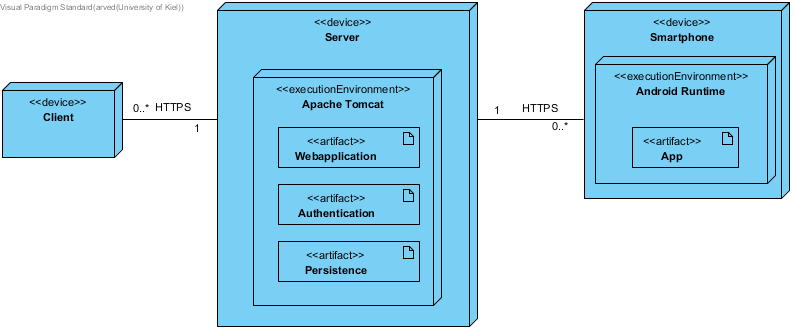
\includegraphics[keepaspectratio,width=15cm]{verteilungsdiagramm/verteilungsdiagramm}
	\caption{Verteilungsdiagramm}
	\label{fig:verteilungsdiagramm}
\end{figure}
In dem Verteilungsdiagramm beschreiben wir welche Komponente auf welcher Hardware installiert wird.
\\
Unsere Webapplikation kommuniziert via HTTPS mit den beiden Clients.
Diese sind einmal ein Benutzer PC, auf dem die Webseite als .html Datei läuft und ein Smartphone mit der Ausführungsumgebung Android Runtime, auf dem die App als .apk installiert wird.
Auf unserem Server läuft die Ausführungsumgebung Apache Tomcat.
Hier läuft die Webapplikation als .war, die Authentifikation und die Persistenz des Spring Frameworks.

		
	\chapter{Klassendiagramme}\label{chp:klassendiagramme}
	\thispagestyle{fancy}
	\section{Server}
\subsection{Model}
\begin{figure}[h]
	\centering
	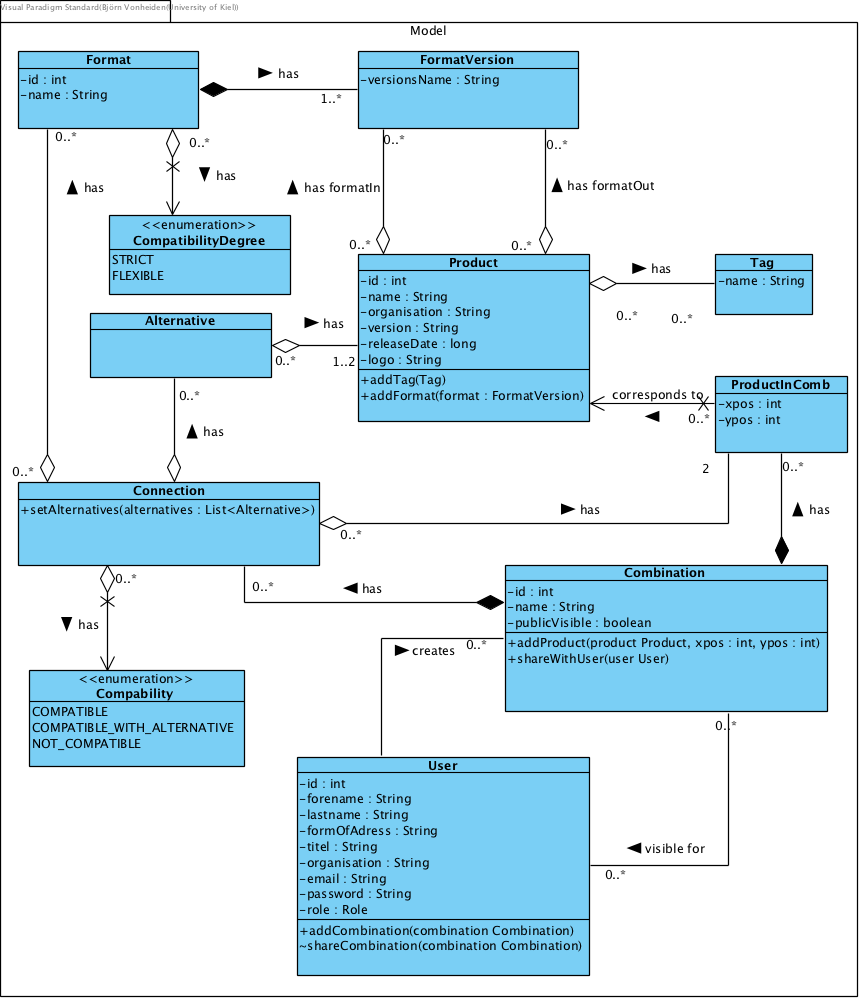
\includegraphics[width=\textwidth]{klassendiagramm/Model}
	\caption{Klassendiagramm - Server - Model}
	\label{fig:klassendiagramm-server-model}
\end{figure}
\begin{table}[h]
	\centering

	\begin{tabularx}{\textwidth}{X X}
		\rowcolor[HTML]{C0C0C0}
		\textbf{Klassenname} & \textbf{Aufgabe} \\
		Model.Alternative & Eine Alternative zu einer Verbindung besteht entweder aus einem oder aus zwei Produkten, welche die Verbindung gültig machen. \\
    	\rowcolor[HTML]{E7E7E7}
    	Model.Combination & Informationen von einer Kombination und Personen, für die die Kombination freigegeben wurde. \\
		Model.Compability  &  Ein Enum, welcher darstellt, ob eine Verbindung kompatibel ist, nicht kompatibel ist oder über eine alternative Kompatibel ist. \\
    	\rowcolor[HTML]{E7E7E7}
		Model.CompatibilityDegree & Ein Enum, welcher entweder 'STRICT' oder 'FLEXIBLE' ist.
		Flexibel heißt, dass das Format abwärts kompatibel ist, strict heißt, dass nur das genau gleiche Format kompatibel ist.\\
		Model.Connection  & Informationen von einer Verbindung. Eine Verbindung hat zwei zugehörige Produkte und eine Richtung.
		Die Richtung wird durch die Reihenfolge der beiden Produkte definiert. \\
    	\rowcolor[HTML]{E7E7E7}
		Model.Format & Ein Format hat eine oder mehrere Versionen und kann entweder strict oder flexible sein. \\
		Model.FormatVersion  & Informationen einer Format-Version.
		Jede Version ist einem Format zugeordnet und hat eine Liste der zugehörigen Produkte, da dies die Suche nach Alternativen effizienter macht.\\
    	\rowcolor[HTML]{E7E7E7}
    	Model.Product & Informationen von einem Dienst.
    	Das Logo wird dabei durch einen Dateipfad definiert. \\
		Model.ProductInComb & Speichert den Ort eines Produktes in einer bestimmten Kombination.
		In einer Kombination kann der selbe Dienst mehrmals vorkommen, dies sind dann aber unterschiedliche ProductInCombs. \\
    	\rowcolor[HTML]{E7E7E7}
		Model.Tag & Ein Tag kann Produkten zugeordnet werden.
		Mithilfe dieser Tags kann nach Produkten gesucht werden. \\
		Model.User & Speichert die Daten eines Benutzers, dessen Combinationen und seine Rolle \\
	\end{tabularx}
	\caption{Klassenbeschreibung - Model}
	\label{table:klassenbeschreibung-model}
\end{table}

\FloatBarrier
\subsection{Logik}
\begin{figure}[h]
	\centering
	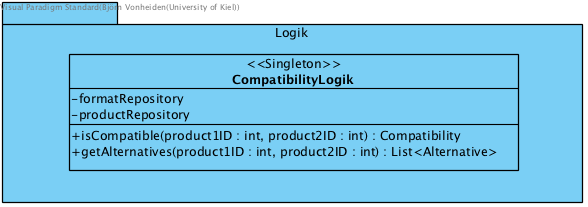
\includegraphics[width=\textwidth]{klassendiagramm/Logik}
	\caption{Klassendiagramm - Logik}
	\label{fig:klassendiagramm-logik}
\end{figure}
\begin{table}[h]
	\centering
	\begin{tabularx}{\textwidth}{X X}
		\rowcolor[HTML]{C0C0C0}
		\textbf{Klassenname} & \textbf{Aufgabe} \\
		Logik.CompatibilityLogik & Diese Klasse bietet Methoden an, um die Kompatibilität zweier Dienste zu prüfen und eine Liste an Alternativen zu bekommen. Die Repository Variablen werden durch die Autowired-Annotation von Spring initialisiert. \\
	\end{tabularx}
	\caption{Klassenbeschreibung - Logik}
	\label{table:klassenbeschreibung-logik}
\end{table}
\FloatBarrier

Im 'Logik' Package sollen alle komplexeren Berechnungen die über die einfache Logik eines Controller hinausgeht.
Als Beispiel für eine solche Berechnung haben wir hier die Kompatibilitätsberechung dargestellt.
Auch die Berechnung der Alternativen für eine inkompatible Verbindung wäre ein solches Beispiel.
Wahrscheinlich werden in diesem Package später auch noch weitere Aufgaben erledigt, wie beispielsweise die Erstellung von JSON-Dateien beziehungsweise von Objekten, welche sich von den Objekten im Model unterscheiden und besser zum Verschicken geeignet sind.
Zudem können noch Methoden dazukommen, welche Informationen aus JSON-Dateien auslesen und an das Modell weiterreichen.



\newpage
\subsection{Controller}
\begin{figure}[h]
	\centering
	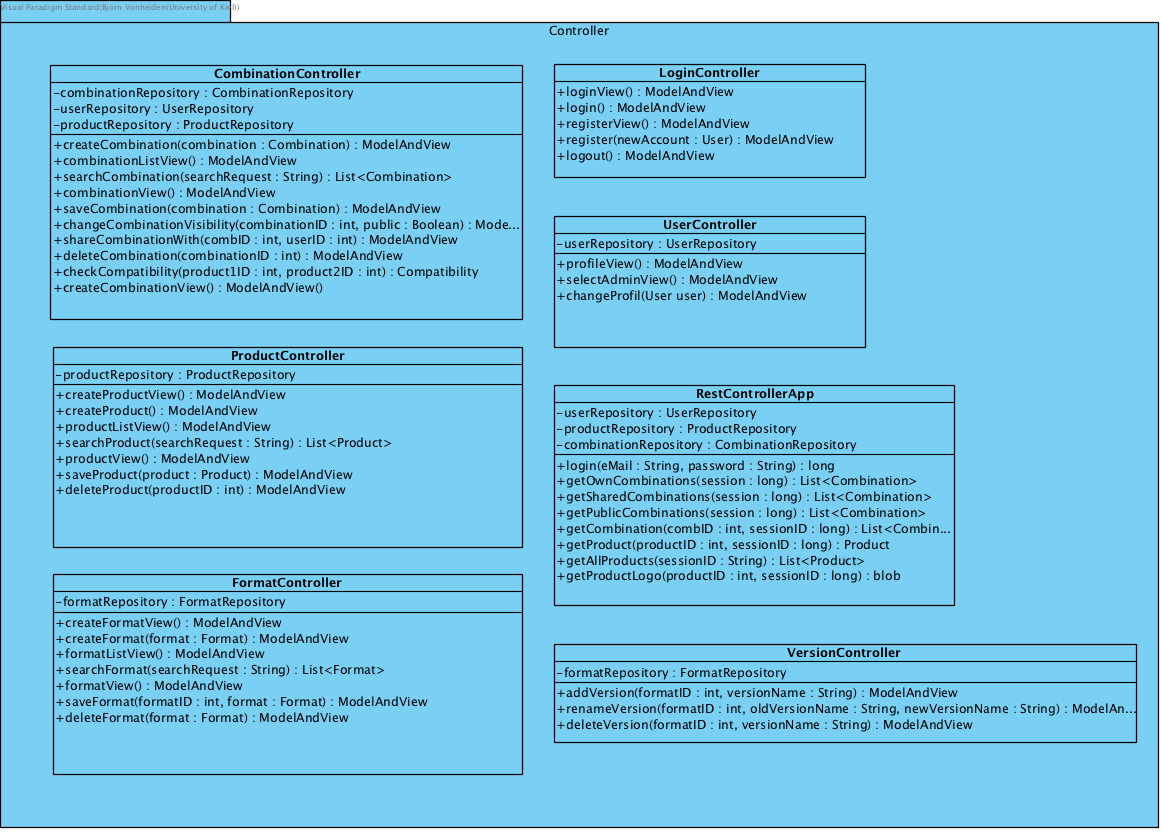
\includegraphics[width=\textwidth]{klassendiagramm/Controller}
	\caption{Klassendiagramm - Controller}
	\label{fig:klassendiagramm-controller}
\end{figure}

\begin{table}[h]
	\centering
	\begin{tabularx}{\textwidth}{X X}
		\rowcolor[HTML]{C0C0C0}
		\textbf{Klassenname} & \textbf{Aufgabe} \\
		Controller.CombinationController & Hier sind alle Controller zur Webapplikation enthalten, welche etwas mit Kombinationen zu tun haben.
		Die Methoden, welche ModelAndView returnen, haben die Annotation '@Controller' und die anderen '@RestController'.
		Die Repositories sind autowired.  \\
		\rowcolor[HTML]{E7E7E7}
		Controller.FormatController  & Diese Klasse enthält alle Controller zur Webapplikation, welche etwas mit Formaten zu tun haben. \\
    	Controller.LoginController & Diese Klasse enthält alle Controller zur Webapplikation, welche etwas mit dem Login zu tun haben.\\
		\rowcolor[HTML]{E7E7E7}
		Controller.ProductController & Diese Klasse enthält analog zur oberen Klasse alle Controller zur Webapplikation, welche etwas mit Diensten zu tun haben. \\
		Controller.RestControllerApp & Diese Klasse enthält alle Controller, welche mit der App kommunizieren.
		Die App schickt dabei GET Anfragen und die URLs fangen mit /App/ an.
		Die Controller sind mit '@RestController' annotiert, es werden also nicht wie bei der Webseite ModelAndViews returnt, sondern in JSON verpackte 		Objekte.
		Die Umwandlung wird von Spring übernommen. \\
		\rowcolor[HTML]{E7E7E7}
		Controller.UserController  & Diese Klasse enthält alle Controller zur Webapplikation, welche etwas mit Benutzern zu tun haben.\\
		Controller.VersionController  & Diese Klasse enthält alle Controller zur Webapplikation, welche etwas mit Versionen von Formaten zu tun haben.\\
		\rowcolor[HTML]{E7E7E7}
	\end{tabularx}
	\caption{Klassenbeschreibung - Controller}
	\label{table:klassenbeschreibung-controller}
\end{table}
\FloatBarrier
\subsection{Repository}
Zusätzlich zu dem 'Model' Package haben wir ein 'Repository' Package, welches zu den Klassen des Models (z.B.: Product) jeweils ein Interface (z.B.: ProductRepository), welches CrudRepository extended.
Die Funktion dieser Interfaces ist die Festlegung der Zugriffsarten auf das Model.
 Da ein Klassendiagramm dazu aber sehr redundant zu dem Model ist und die konkreten Methoden von der Implementierung der Controller abhängig ist, haben wir das hier weggelassen.

\FloatBarrier
\subsection{Security}
In dem 'Security'-Package sollen die Funktionen der Authentification \& Authorization umgesetzt werden. Da viele Funktionen und Klassen schon durch das Spring-Security-Framework gestellt werden und nur konfiguriert bzw. aufgerufen werden müssen und wir uns der Umsetzung noch nicht komplett klar sind, haben wir ein Diagramm an dieser Stelle weggelassen.
So werden wir voraussichtlich beispielsweise für die Http-Requests vorkonfigurieren welche Rollen (siehe Model - User), welche Requests stellen darf.
So unterscheiden wir die Rollen, wie im Pflichtenheft, in unangemeldete Nutzer, eingeloggte Nutzer und Administratoren.
So werden die Seiten: Kombinationen(nur mit den freigegebenen Kombinationen), Dienste, Login und Registrieren, für alle Nutzer freigeben.
Die Seiten: Kombinationen(mit den zusätzlichen Optionen eigene und für einen Freigegebene), Profil und Logout sind für alle angemeldeten Nutzer freigegeben.
Diese erhalten dabei auch Zugriff auf weitere Funktionen wie das Speichern einer Kombination.
Für Administratoren werden zusätzlich noch die Seite Benutzer freigegeben.
Außerdem wird ihm noch der Zugriff auf Administrator-Funktionen wie das Hinzufügen oder Löschen eines Dienstes.
An den meisten Methoden werden wir den Sicherheitsaspekt durch die Security-Annotations des Spring Frameworks umsetzen.


\newpage
\section{App}
\begin{figure}[h]
	\centering
	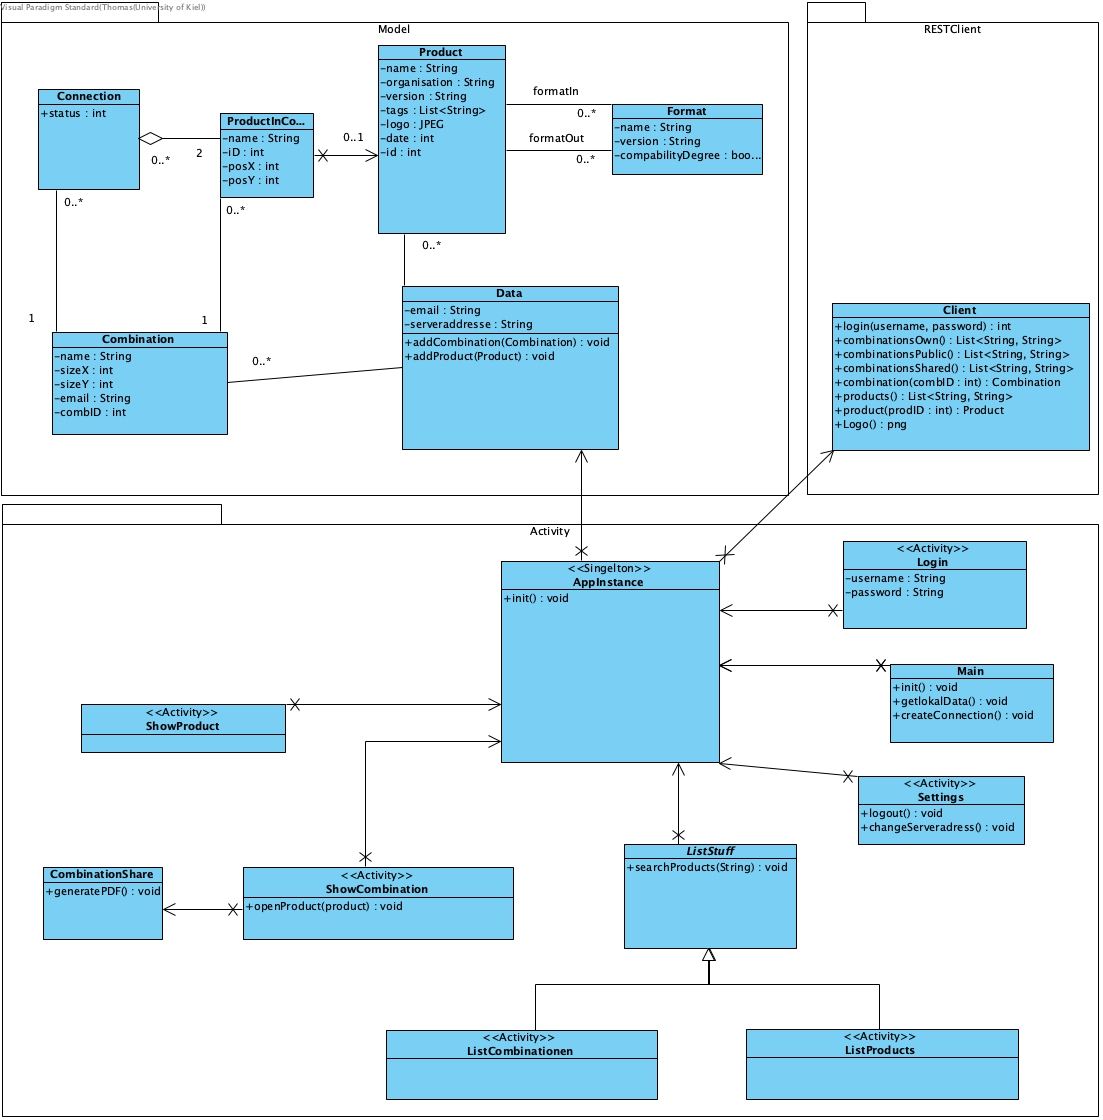
\includegraphics[width=\textwidth]{klassendiagramm/App}
	\caption{Klassendiagramm - App}
	\label{fig:klassendiagramm-app}
\end{figure}

\begin{table}[h]
	\centering
	\begin{tabularx}{\textwidth}{X X}
		\rowcolor[HTML]{C0C0C0}
		\textbf{Klassenname} & \textbf{Aufgabe} \\
		AppInstance & Singelton erlaubt Zugriff auf Data und Client\\
		\rowcolor[HTML]{E7E7E7}
		Client & Übernimmt alle Kommunikationen mit dem Server \\
		CombinationShare & Leitet PDF an das Android System weiter \\
		\rowcolor[HTML]{E7E7E7}
		DataManagement.Combination & Informationen von einer Kombination \\
		DataManagement.Connection  & Informationen von einer Verbindung \\
		\rowcolor[HTML]{E7E7E7}
		DataManagement.Data & Speichert lokal relevante Daten \\
		DataManagement.Format  & Informationen eines Formats\\
		\rowcolor[HTML]{E7E7E7}
		DataManagement.Product & Informationen von einem Dienst \\
		DataManagement.ProductInComb & Speichert ausschließlich die Informationen eines Produkts die zum Visualisieren der Kombination relevant sind.\\
		\rowcolor[HTML]{E7E7E7}
		ListCombination & Darstellung aller möglichen Kombinationen und diese suchbar machen\\
		ListProducts & Darstellung aller möglichen Dienste und diese suchbar machen\\
		\rowcolor[HTML]{E7E7E7}
		ListStuff & Abstrakte Klasse für die Listen(Dienste und Kombinationen)\\
		Login & Stellt den Login bereit \\
		\rowcolor[HTML]{E7E7E7}
		Main & Initialisiert die Applikation \\
		Settings & Stellt Einstellungen für Benutzer bereit \\
    \rowcolor[HTML]{E7E7E7}
		ShowCombination & Generiert Canvas einer Kombination und visualisiert diese  \\
		ShowProduct & Zeigt einen einzelnen Dienst an
	\end{tabularx}
	\caption{Klassenbeschreibung - App}
	\label{table:klassenbeschreibung-app}
\end{table}

	
	\chapter{Sequenzdiagramme}\label{chp:sequenzdiagramme}
	\thispagestyle{fancy}
	\section{Webseite, Server}

Bei den folgenden Sequenzdiagrammen stellt die RestAPI Klasse das Spring Framework dar, damit wir sowohl die HTML Requests, als auch die Controller Methoden zeigen können.

\begin{figure}[h]
	\centering
	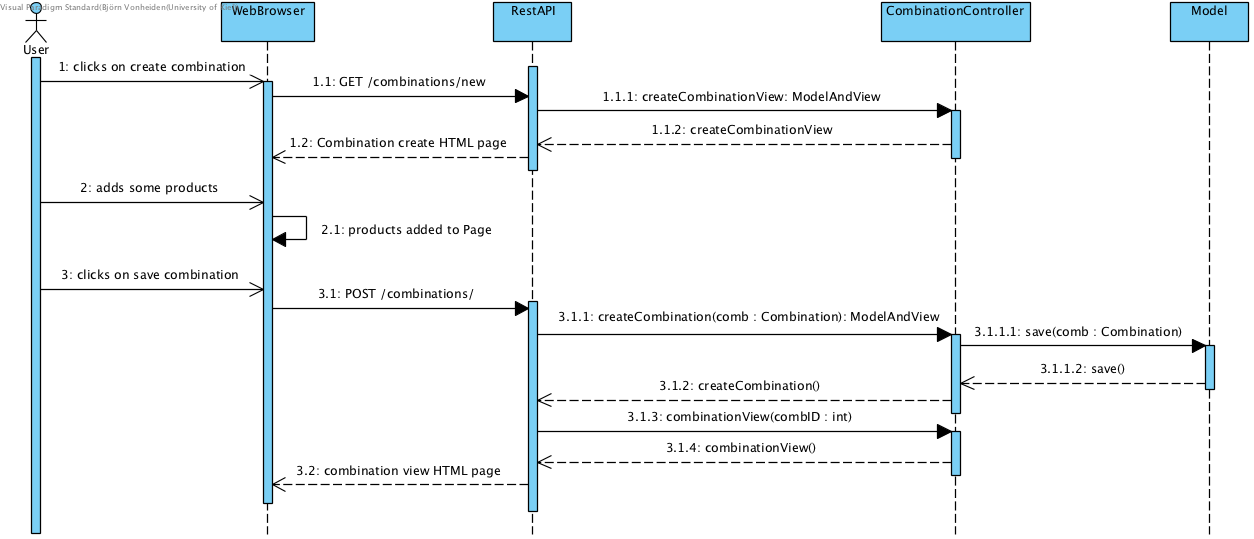
\includegraphics[width=\textwidth]{sequenzdiagramm/Kombination_erstellen}
	\caption{Sequenzdiagramm - Kombination erstellen Webseite}
	\label{fig:sequenz-erstellKombWeb}
\end{figure}
\FloatBarrier
In der Abbildung \ref{fig:sequenz-erstellKombWeb} wird dargestellt, wie man auf der Webseite eine Kombination erstellen kann.
Dabei wird in diesem Fall nur berücksichtigt, dass der Benutzer ein paar Dienste zu der Kombination hinzufügt, aber keine Kompatibilitätsprüfung ausführt.
Eine Kompatibilitätsprüfung wird in dem Sequenzdiagramm \ref{fig:sequenz-freiKombWeb} ausgeführt.\\
Der Benutzer klickt, um eine neue Kombination zu erstellen, auf einen Button.
Dafür wird dann eine neue Webseite von dem Server angefragt.
Im Browser kann der Benutzer dann einzelne Dienste der Kombination hinzufügen.
Wenn er dann fertig ist, klickt er auf Kombination speichern.
Dadurch schickt der Browser einen POST Request mit den entsprechenden Daten an die API.
Auf dem Server wird daraufhin die Kombination gespeichert.
Der CombinationController führt dann ein redirect aus, um auf die Webseite zu gelangen, wo die Kombination dann angezeigt wird.


\begin{figure}[h]
	\centering
	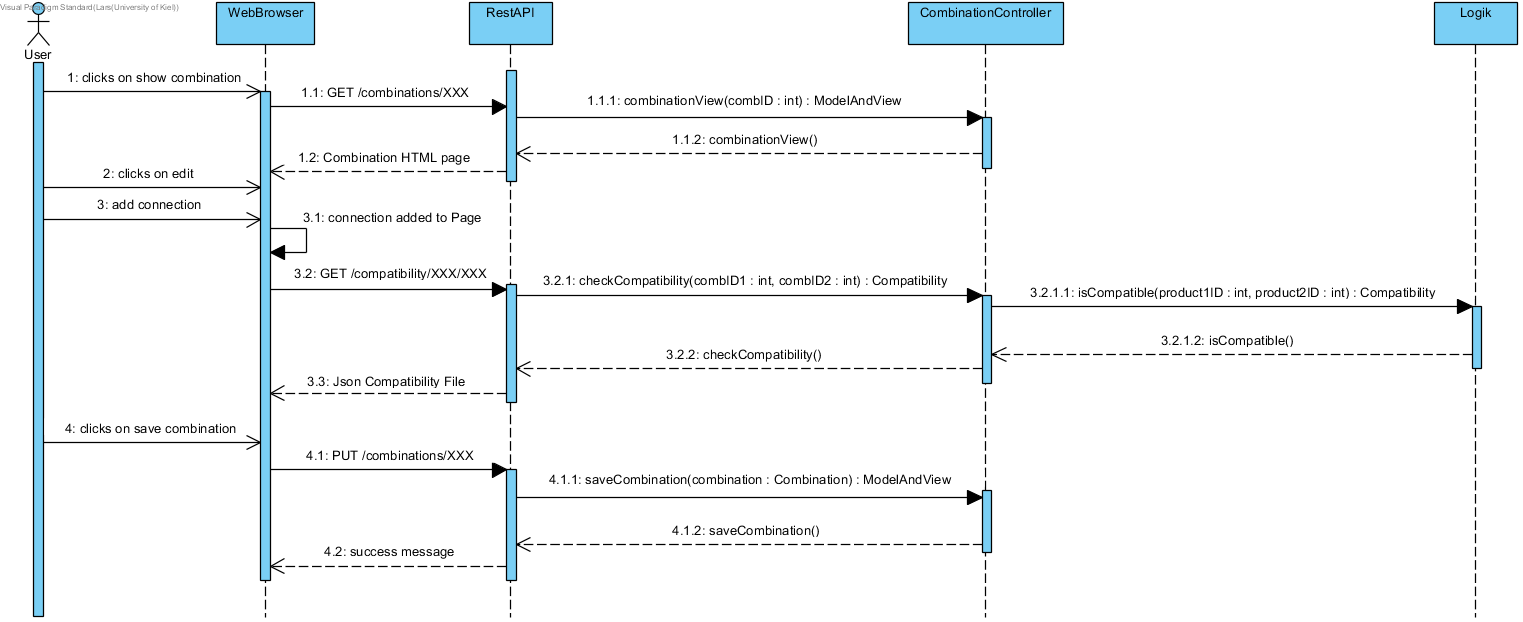
\includegraphics[width=\textwidth]{sequenzdiagramm/Kombination_bearbeiten}
	\caption{Sequenzdiagramm - Kombination bearbeiten Webseite}
	\label{fig:sequenz-bearbKombWeb}
\end{figure}
\FloatBarrier
In der Abbildung \ref{fig:sequenz-bearbKombWeb} lässt sich der Benutzer eine seiner Kombinationen anzeigen und bearbeitet dann diese Kombination.
Die Kombination soll bereits mindestens zwei nicht verbundene Dienste enthalten.
Dann fügt er dort eine Verbindung zwischen zwei Diensten ein. \\
Als erstes öffnet der Benutzer eine seiner Kombinationen.
Dafür wird eine Anfrage an den Server geschickt und dieser gibt eine HTML-Seite zurück.
Der Benutzer, klickt dann auf Kombination editieren.
Im Browser hat er dann die Möglichkeit seine Kombination zu bearbeiten.
Dort fügt er dann eine Verbindung zwischen zwei Kombinationen ein.
Der Browser schickt dadurch dann eine Anfrage an den Server.
Der Controller, der die Anfrage entgegennimmt, leitet die Überprüfung an die Logik weiter.
Wenn der Controller dann eine Antwort bekommt, wird diese als JSON zurück an den Browser gegeben.


\begin{figure}[h]
	\centering
	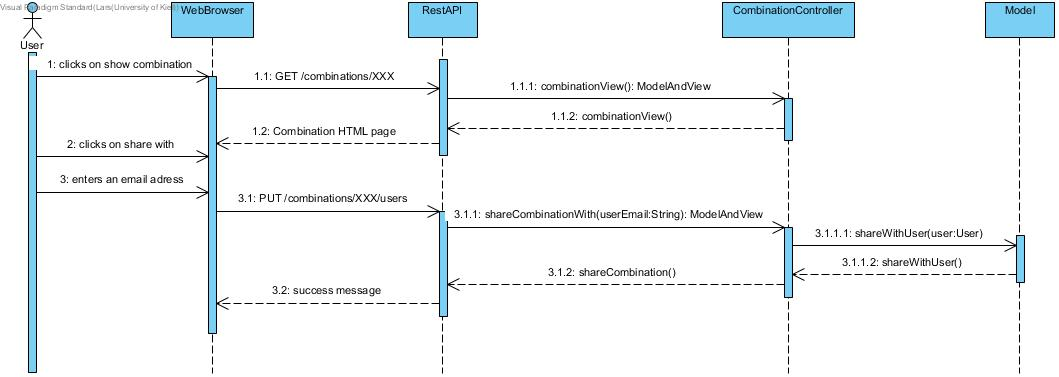
\includegraphics[width=\textwidth]{sequenzdiagramm/Kombination_freigeben}
	\caption{Sequenzdiagramm - Kombination freigeben Webseite}
	\label{fig:sequenz-freiKombWeb}
\end{figure}
\FloatBarrier
In der Abbildung \ref{fig:sequenz-freiKombWeb} wird das Freigeben einer eigenen Kombination an einen anderen Nutzer dargestellt.
Anschließend kann der andere Nutzer diese Kombination ebenfalls ansehen, allerdings nicht bearbeiten.
Zunächst wird wie im Diagramm \ref{fig:sequenz-bearbKombWeb} eine Kombination angezeigt.
Im Browser kann der Nutzer nun auf freigeben klicken und eine E-Mail Adresse eingeben.
Diese wird über einen HTTP PUT Request an den Server geschickt.
Dort macht der entsprechende Controller eine Anfrage an das Model, wodurch der Nutzer zu den Personen mit Zugriffsrechten auf die Kombination hinzugefügt wird.
Falls der andere Nutzer nun auf der Webseite eine GET /combinations oder auf der App eine GET /app/combinations/shared Anfrage macht, wird diese Kombination zusätzlich angezeigt.

\begin{figure}[h]
	\centering
	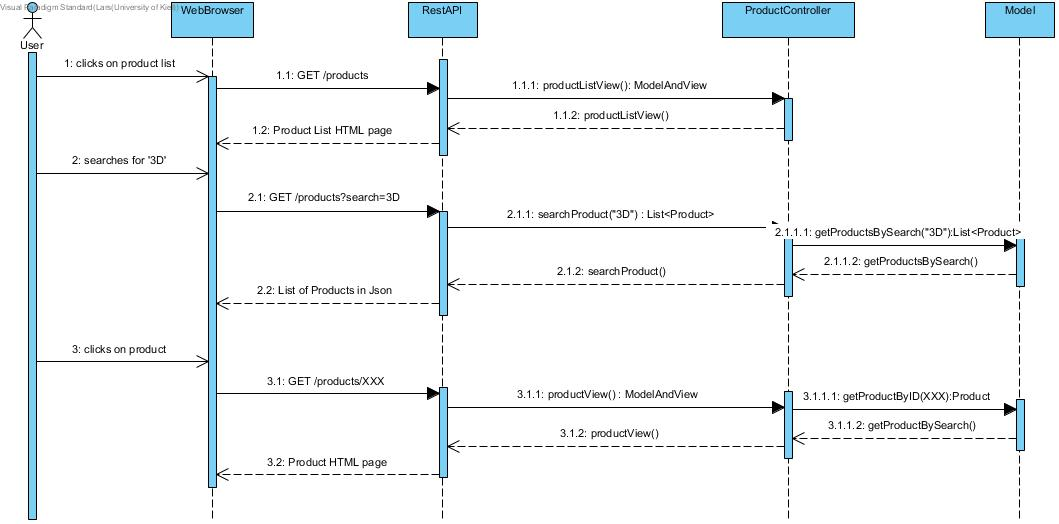
\includegraphics[width=\textwidth]{sequenzdiagramm/Dienstsuchen}
	\caption{Sequenzdiagramm - Dienst Suchen Webseite}
	\label{fig:sequenz-suchDienstWeb}
\end{figure}
\FloatBarrier

In der Abbildung \ref{fig:sequenz-suchDienstWeb} wird die Suche und das Anzeigen eines Dienstes gezeigt. Zunächst werden alle Produkte geladen, für eine Übersicht.
Bei der anschließenden Suche wird der Suchbegriff in der URL weitergegeben.
Der Controller macht dann eine Anfrage, welche im Repository definiert ist.
Dabei wird sowohl nach einem Tag, als auch dem Dienstnamen gesucht und die jeweiligen Dienste werden aus dem Model geholt.
Da die Methoden aber über Spring laufen, haben wir es im Diagramm direkt an das Model geschickt.
Anschließend erhält der Nutzer die Dienste und kann über eine weitere Anfrage einen Dienst öffnen.


\section{App}
\begin{figure}[h]
	\centering
	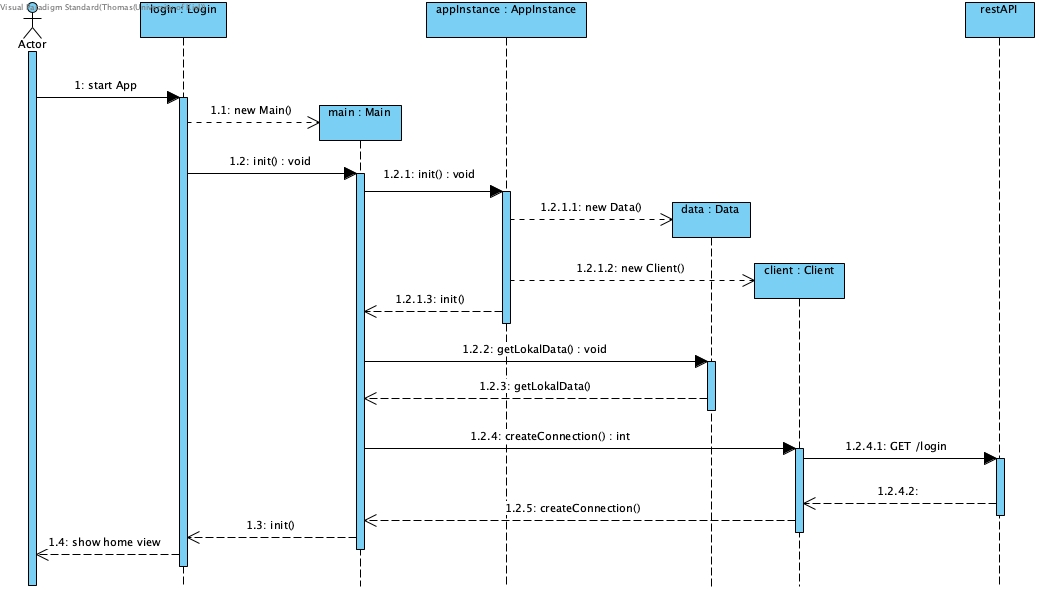
\includegraphics[keepaspectratio,width=\textwidth]{sequenzdiagramm/AppStartUp}
	\caption{Sequenzdiagramm - App Start-Up}
	\label{fig:sequenz-appstartup}
\end{figure}
\FloatBarrier
In der Abbildung \ref{fig:sequenz-appstartup} wird der Ablauf des Start-up der App abgebildet. Es wird dargestellt wie die wichtigen Klassen initialisiert werden und wie die Verbindung zum Server aufgebaut bevor der Login Bildschirm angezeigt wird.

\begin{figure}[h]
	\centering
	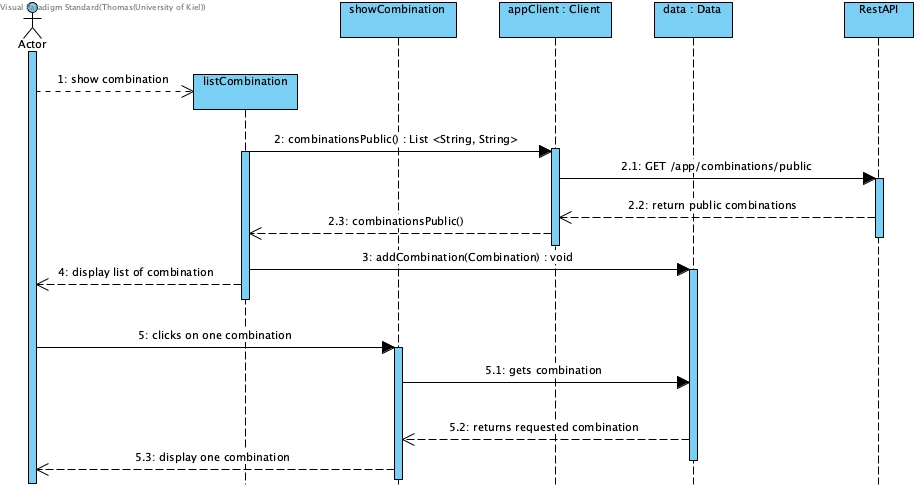
\includegraphics[width=\textwidth]{sequenzdiagramm/ShowCombinationohneAcc}
	\caption{Sequenzdiagramm - Kombinationen anzeigen ohne Account}
	\label{fig:sequenz-appohneaccount}
\end{figure}
\FloatBarrier
In der Abbildung \ref{fig:sequenz-appohneaccount} wird das Anzeigen von öffentlichen Kombinationen modelliert. Benutzer ohne eigenen Account haben nur die Option öffentlich geteilte Kombinationen anzusehen. Der Client der App holt sich mit der GET combinations/public Anfrage alle öffentlich verfügbaren Kombinationen. Diese werden zurück an die App übertragen, damit sie dem Nutzer zugänglich gemacht werden können.

\begin{figure}[h]
	\centering
	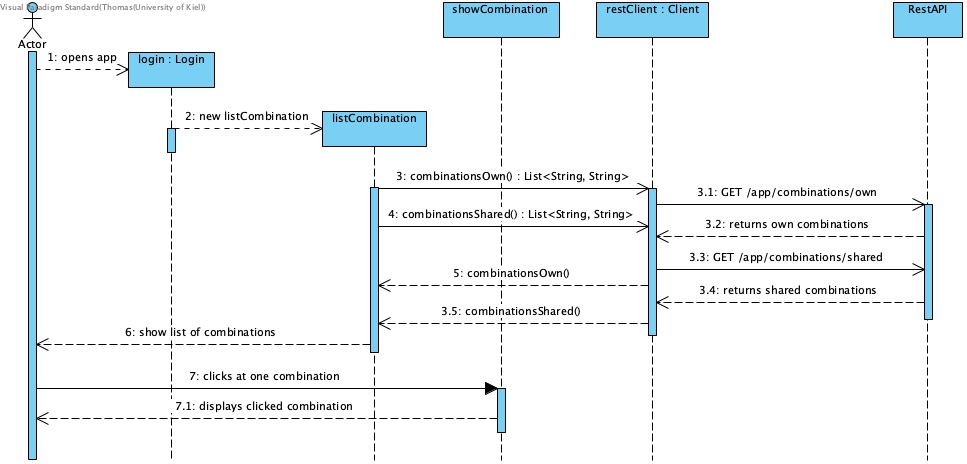
\includegraphics[width=\textwidth]{sequenzdiagramm/ShowCombinationWithAcc}
	\caption{Sequenzdiagramm - Kombinationen anzeigen mit Account}
	\label{fig:sequenz-ShowMitAccount}
\end{figure}
\FloatBarrier
In Abbildung \ref{fig:sequenz-ShowMitAccount} wird der Ablauf dargestellt, wenn ein eingeloggter User seine eigenen Kombinationen ansehen will. Zusätzlich wird die Liste auch mit den Kombinationen erweitert, die für den User freigegeben worden sind. Hier stellt der Client neben der GET combinations/own Anfrage auch eine combinations/shared Anfrage, da Nutzer mit eigenen Account auch die Kombinationen der eigenen Organisation oder von anderen Nutzern freigegebene Kombinationen ansehen kann. Die übertragenen Kombinationen tauchen auch wieder in einer Liste von möglichen Kombinationen auf.

\begin{figure}[h]
	\centering
	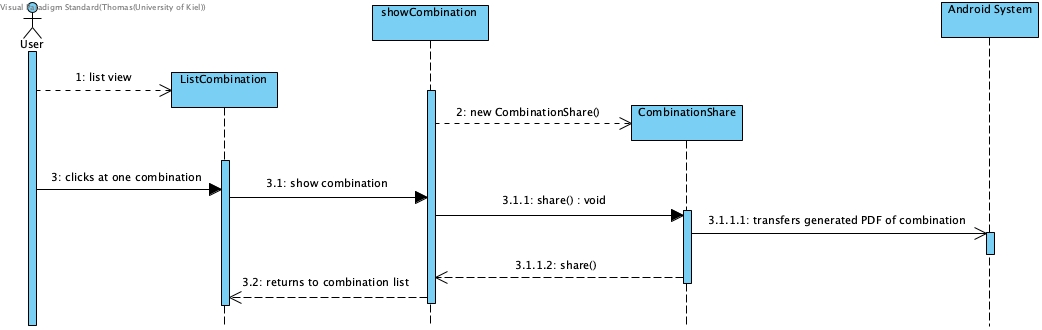
\includegraphics[width=\textwidth]{sequenzdiagramm/Kombinationteilen}
	\caption{Sequenzdiagramm - Kombination teilen}
	\label{fig:sequenz-kombTeilen}
\end{figure}
\FloatBarrier
In der Abbildung \ref{fig:sequenz-kombTeilen}  beschreiben wir die Möglichkeit eine vorhandene Kombination mit dem Standard Mail-Programm auf dem Handy zu versenden. Der Nutzer öffnet die Kombination, die er per Mail versenden möchte. Dort besteht die Möglichkeit die Kombination zu teilen, wodurch sich die Standard Weiterleitung von Android öffnet. Dort werden die Daten an das Mail Programm weitergeleitet. Nach dem Versenden werden dem Nutzer wieder die Liste aller möglichen Kombinationen angezeigt.

	
	\chapter{Rest Api}\label{chp:restapi}
	\thispagestyle{fancy}
	\section{Webseite}
\begin{table}[h]
	\centering
	\begin{tabularx}{\textwidth}{l l l l}
		\rowcolor[HTML]{C0C0C0}
		\textbf{Methode} & \textbf{URL} & \textbf{Server Klasse} & \textbf{Server Methode}\\
		\\
		\multicolumn{4}{c}{\textbf{Seiten}}\\
		\rowcolor[HTML]{E7E7E7}
		GET & /register & LoginController & registerView \\
		GET & /login & LoginController & loginView \\
		\rowcolor[HTML]{E7E7E7}
		GET & /combinations & CombinationController & combinationListView \\
		GET & /combinations/XXX & CombinationController & combinationView \\
		\rowcolor[HTML]{E7E7E7}
		GET & /products & ProductController & productListView \\
		GET & /products/XXX & ProductController & productView \\
		\rowcolor[HTML]{E7E7E7}
		GET & /formats/ & FormatController & formatListView \\
		GET & /formats/XXX & FormatController & formatView \\
		\rowcolor[HTML]{E7E7E7}
		GET & /users/XXX  & UserController & profileView \\
		GET & /admin & UserController & selectAdminView \\
		\rowcolor[HTML]{E7E7E7}
		GET & /combinations/new & CombinationController & createCombinationView \\
		GET & /formats/new & FormatController & createFormatView \\
		\rowcolor[HTML]{E7E7E7}
		GET & /products/new & ProductController & createProductView \\
		\\
		\multicolumn{4}{c}{\textbf{Suchen}}\\
		GET & /products?search=XXX & ProductController & searchProduct \\
		\rowcolor[HTML]{E7E7E7}
		GET & /combinations?search=XXX & CombinationController & searchCombination \\
		GET & /formats?search=XXX & FormatController & searchFormat \\
		\\
		\multicolumn{4}{c}{\textbf{Erstellen}}\\
		\rowcolor[HTML]{E7E7E7}
		POST & /users & UserController & register \\
		POST & /products & ProductController & createProduct \\
		\rowcolor[HTML]{E7E7E7}
		POST & /formats & FormatController & createFormat \\
		POST & /combinations & CombinationController & createCombination \\
		\rowcolor[HTML]{E7E7E7}
		POST & /formats/XXX/version & VersionController & addVersion \\
		\\
		\multicolumn{4}{c}{\textbf{Update}}\\
		PUT & /users/XXX & UserController & changeUser \\
		\rowcolor[HTML]{E7E7E7}
		PUT & /combinations/XXX & CombinationsController & saveCombination \\
		PUT & /combinations/XXX/visibility & CombinationsController & changeCombinationsVisibility \\
		\rowcolor[HTML]{E7E7E7}
		PUT & /combinations/XXX/users & CombinationsController & shareCombinationWith \\
		PUT & /products/XXX & ProductController & saveProduct \\
		\rowcolor[HTML]{E7E7E7}
		PUT & /formats/XXX & FormatController & saveFormat \\
		PUT & /users/XXX/version/XXX & VersionController & renameVersion \\
		\\
		\multicolumn{4}{c}{\textbf{Löschen}}\\
		\rowcolor[HTML]{E7E7E7}
		DELETE & /combinations/XXX & CombinationsController & deleteCombination \\
		DELETE & /products/XXX & ProductController & deleteProduct \\
		\rowcolor[HTML]{E7E7E7}
		DELETE & /formats/XXX & FormatController & deleteFormat \\
		DELETE & /formats/XXX/version/XXX & VersionController & deleteVersion \\
		\\
		\multicolumn{4}{c}{\textbf{Sonstiges}}\\
		\rowcolor[HTML]{E7E7E7}
		GET & /compatibility/XXX/XXX & CombinationsController & checkCompatibility \\
		GET & /login/XXX & LoginController & login \\
		\rowcolor[HTML]{E7E7E7}
		GET & /logout/XXX & LoginController & logout \\

	\end{tabularx}
	\caption{Rest - Webseite}
	\label{table:rest-webseite}
\end{table}


\section{App}
\begin{table}[h]
	\centering
	\begin{tabularx}{\textwidth}{l l l l}
		\rowcolor[HTML]{C0C0C0}
		\textbf{Methode} & \textbf{URL} & \textbf{Server Klasse} & \textbf{Server Methode} \\
		\rowcolor[HTML]{E7E7E7}
		GET & /app/combinations/own & RestControllerApp & getOwnCombinations \\
		GET & /app/combinations/shared & RestControllerApp & getSharedCombinations \\
		\rowcolor[HTML]{E7E7E7}
		GET & /app/combinations/public & RestControllerApp & getPublicCombinations \\
		GET & /app/combinations/XXX & RestControllerApp & getCombination \\
		\rowcolor[HTML]{E7E7E7}
		GET & /app/products & RestControllerApp & getAllProducts \\
		GET & /app/products/XXX & RestControllerApp & getProduct \\
		\rowcolor[HTML]{E7E7E7}
		GET & /app/products/XXX/Logo & RestControllerApp & getProductLogo \\

	\end{tabularx}
	\caption{Rest - App}
	\label{table:rest-app}
\end{table}

\section{Erklärung}
Bei der Webseite wird grundsätzlich ein ModelAndView zurückgegeben, die View ist dabei die neue HTML Seite und das Model enthält die benötigten Daten.
Es gibt aber auch Ausnahmen: Beispielsweise bei der Suche nach Diensten wird nur eine Liste von Diensten (über JSON) zuückgegeben, da sich die View nicht ändert und man sowohl in der Dienst-Liste, als auch bei der Komponentenbearbeitung nach Diensten suchen kann.
Die Methoden, die ModelAndView zurückgeben, haben '@Controller' als Annotation und die anderen '@RestController'.
Die jeweiligen Rückgabearten der Methoden kann man im Klassendiagramm finden.
Bei den Requests von der App ist die URL immer mit '/app/' markiert, die jeweiligen Controller sind mit '@RestController' annotiert.
Die HTTP Methode ist dort immer GET und es werden JSON Objekte im Response Body zuückgegeben.
Allgemein sind die GET Methode für Datenabfrage und neue Views, POST für das erstellen von Objekten, PUT für das ändern von Daten und DELETE zum Löschen von Daten.
Da User nicht gelöscht werden können, haben wir dafür keine Methode.
Der Unterschied zwischen loginView (bzw. registerView) und login (register) ist, dass mit der View Methode nur die Seite zum anmelden oder registrieren angezeigt wird und mit der anderen die Aktion durchgeführt wird.

	
	\chapter{Glossar}\label{chp:glossar}
	\thispagestyle{fancy}
	\begin{table}[h]
	\centering
	\begin{tabularx}{\textwidth}{X X}
		\rowcolor[HTML]{C0C0C0}
		\textbf{Abkürzung} & \textbf{Beschreibung} \\
		API & Application Programming Interface \\
		\rowcolor[HTML]{E7E7E7}
		CPU & Cental Processing Unit \\
		JSON & JavaScript Object Notation \\
		\rowcolor[HTML]{E7E7E7}
		RAM & Random-Access Memory \\
		REST & Representational State Transfer \\
		\rowcolor[HTML]{E7E7E7}
		Lookup-Zeit & Zugriffszeit auf die Daten \\
	\end{tabularx}
	\caption{Glossar}
	\label{table:glossar}
\end{table}

	
	\bibliography{references}
	\pagenumbering{gobble} % Nummerierung deaktivieren
	
\end{document}